El Procesamiento del Lenguaje Natural (PLN) emerge de la combinación entre la inteligencia artificial y la lingüística. A diferencia de las diversas tareas que pueden tratar el aprendizaje automático o el aprendizaje profundo, el pnl se enfoca en tareas relacionadas con cualquier lenguaje o idioma, que los seres humanos utilicen para comunicarse de manera cotidiana, ya sea oral o escrita, este tipo de lenguaje es inherente a las culturas y evoluciona orgánicamente a lo largo del tiempo.

Vajjala define el PLN como ``un área de la informática que se enfoca en métodos para analizar, modelar y comprender el lenguaje humano. Prácticamente toda aplicación inteligente que implica el lenguaje humano tiene raíces en el PLN'' \cite[p. 4]{vajjala2020practical}.
 
El procesamiento del lenguaje natural, el aprendizaje profundo y el aprendizaje automático son subcampos de la Inteligencia Artificial que, de hecho, se superponen  entre ellos, ver Figura \ref{fig:nlp1}.Ya que estas disciplinas colaboran entre sí e incluso sirven como base la una a la otra, como ocurre con el aprendizaje automático y el aprendizaje profundo, e igualmente  muchos modelos de lenguaje hacen uso tanto del aprendizaje profundo como de técnicas tradicionales del aprendizaje automático. Sin embargo esto no evita que cada una de estas disciplinas tenga su área específica de estudio. Como el PLN que, se concentra en el análisis y comprensión del lenguaje humano, explorando diversas técnicas para estos propósitos.

\begin{figure}[h!]
	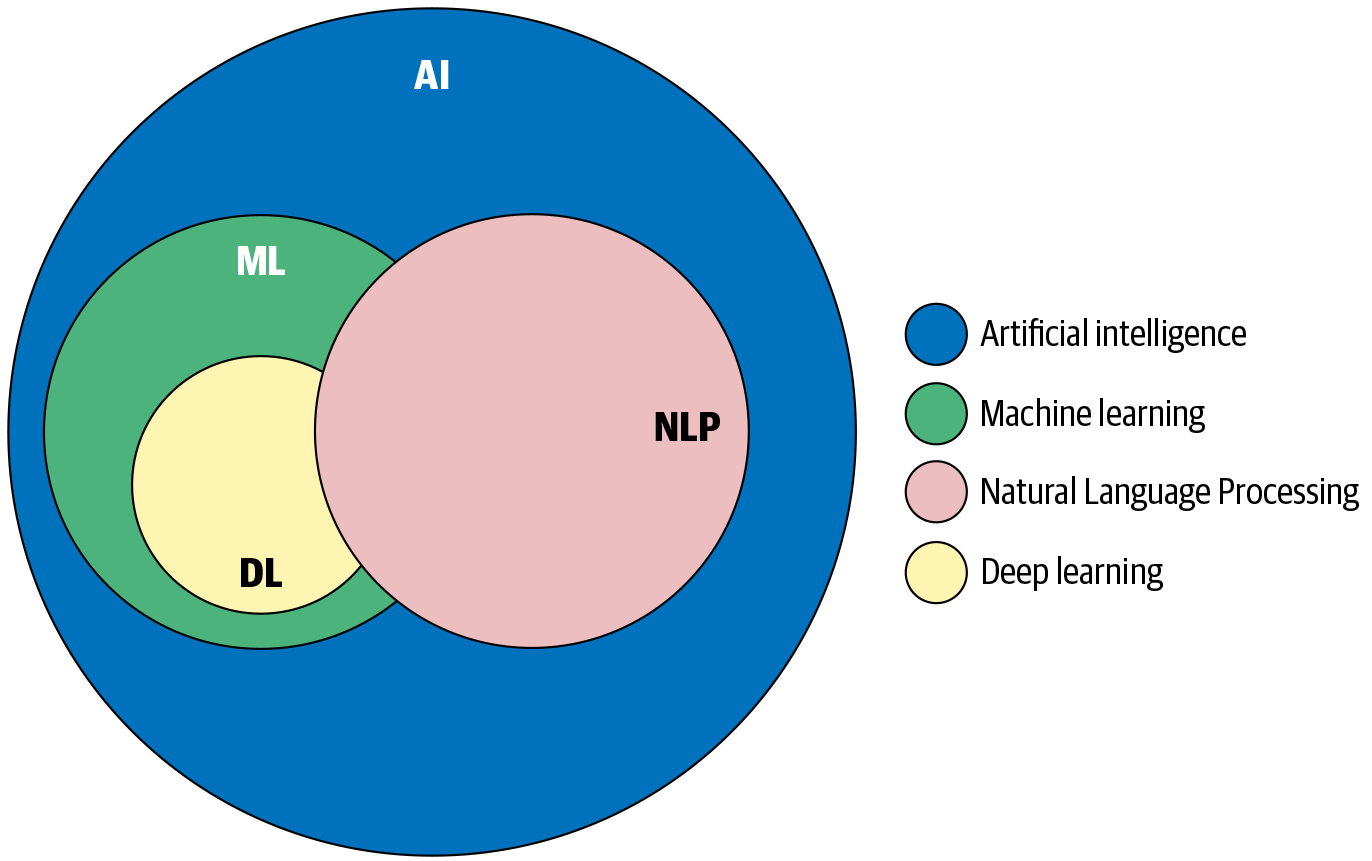
\includegraphics[width=0.65\textwidth]{capitulo3/figuras/nlp1.png}
	\caption[Como NLP, ML, y DL se relacionan]{Como NLP, ML, y DL se relacionan
		\\\textit{Fuente: Extraído de} \protect \cite[p. 15]{vajjala2020practical} } 
	\label{fig:nlp1}
\end{figure}
